\documentclass[a4paper]{report}
\usepackage[latin1]{inputenc}
\usepackage[T1]{fontenc}
\usepackage[francais]{babel}
\usepackage{setspace}
\usepackage{url}
\usepackage{graphicx}

\title{Homework 5 - Lab}
\author{Achille \textsc{Sala\"{u}n}}

\begin{document}
\maketitle

\section*{Question 1}
There are $N=6301$ nodes and $M=20777$ edges in the network.
\medbreak

To create the \textit{adjacency matrix} ADJ, I built the following method : 

\medbreak
\noindent     \textit{\# build the adjacency matrix}\\
\noindent     \texttt{def buildAdjacencyMatrix(gnutella):}\\
\hspace*{1cm} \texttt{	N = numberNodes(gnutella)}\\
\hspace*{1cm} \texttt{	matrix = [[0 for j in range(0,N)] for i in range(0,N)]}\\
\hspace*{1cm} \texttt{	for l in range(0,len(gnutella)):}\\
\hspace*{2cm} \texttt{			line = gnutella[l]}\\
\hspace*{2cm} \texttt{			i = line[0]}\\
\hspace*{2cm} \texttt{			j = line[1]}\\
\hspace*{2cm} \texttt{			matrix[i-1][j-1]=1}\\
\hspace*{2cm} \texttt{			matrix[j-1][i-1]=1}\\
\hspace*{1cm} \texttt{	return matrix}\\
\medbreak

Where the \texttt{gnutella} input is a list of pairs.

%-------------------------------------------------------------------------------------------------------%
\section*{Question 2}
I would choose $p = \frac{d}{N}$, where $d$ is the \textit{average degree} of the network.

%-------------------------------------------------------------------------------------------------------%
\section*{Question 3}

The degree distribution is, we could plot it in the chart of the \textsc{Figure} \ref{fig:total}.
\medbreak

\begin{figure}[!h]
	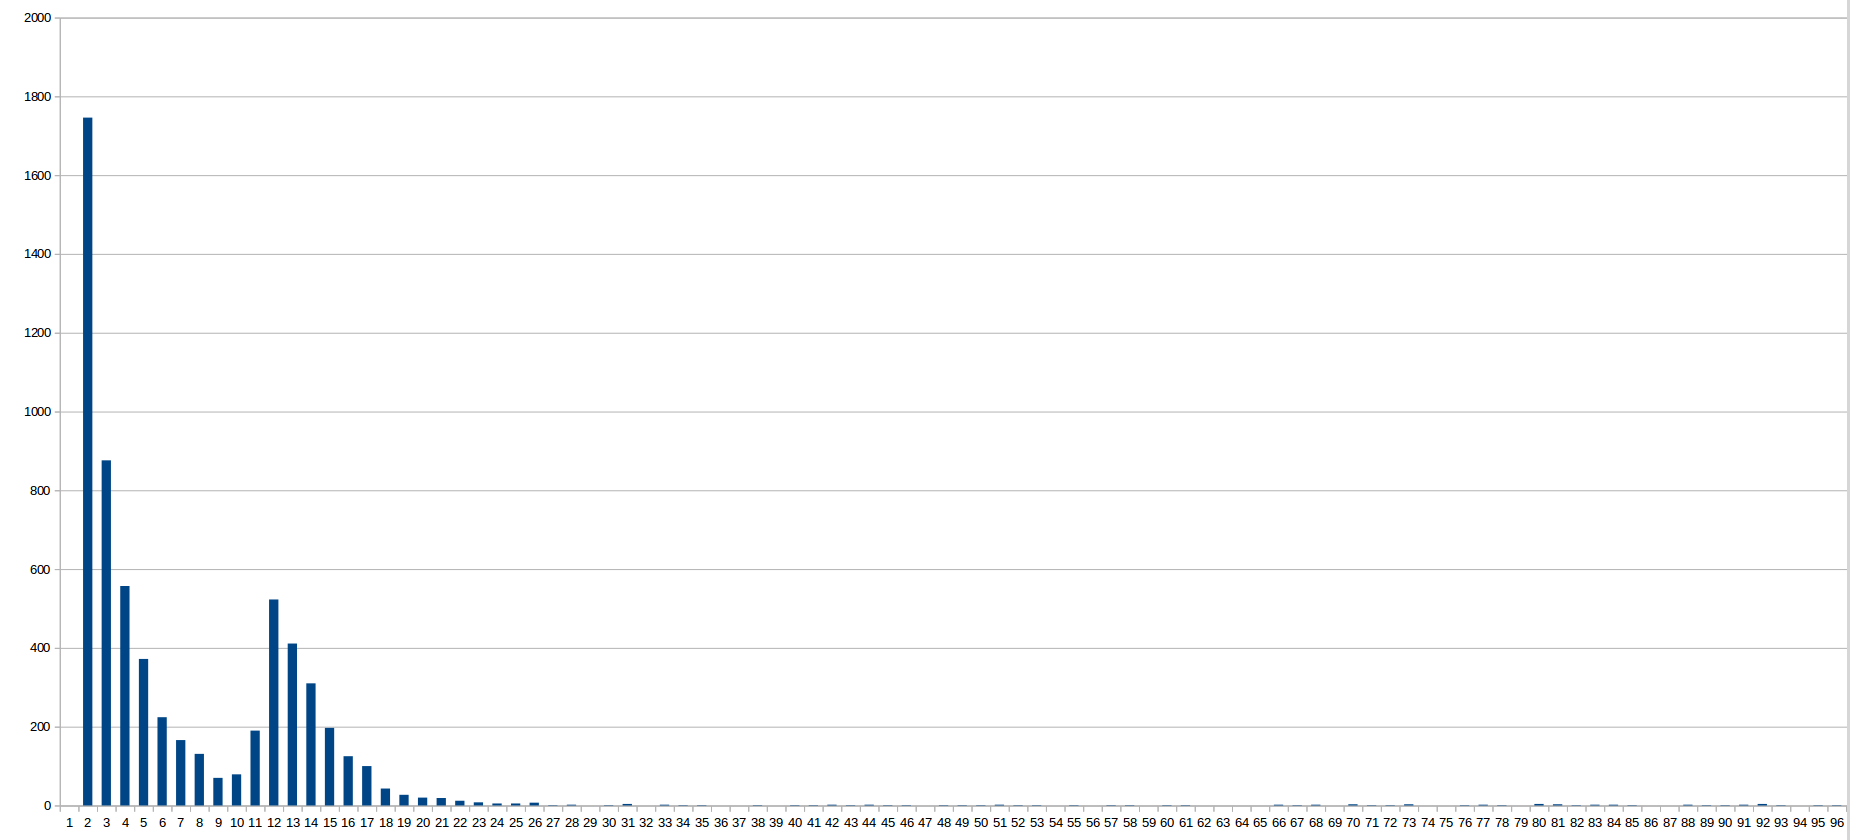
\includegraphics[scale=.17]{./total.png}
	\caption{Degree distribution of the whole network}
	\label{fig:total}
\end{figure}

Furthermore, the \textit{average degree} is $6.595$, the \textit{maximum degree} is $97$, while the \textit{minimum degree} is $1$. 
\medbreak
The degree distribution is not \textit{power-law}, indeed, we can see two local maxima which is not the shape of a power-law degree distribution. \\
When we look at the graph (cf. \textsc{Figure} \ref{fig:graph}), we can see the existence of a "core" : there the average degree is different and explains the second maximum.

\begin{figure}[!h]
	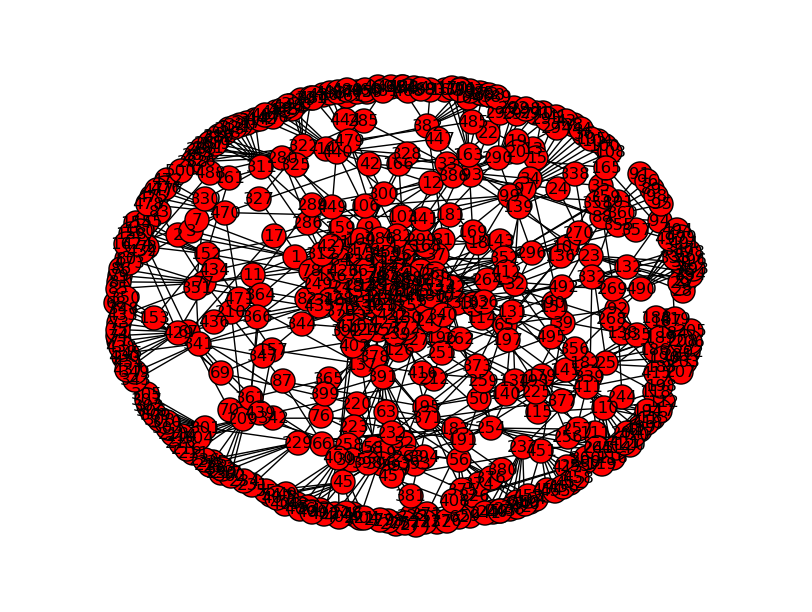
\includegraphics[scale=.6]{./figure_1.png}
	\caption{Subnetwork's whole view}
	\label{fig:graph}
\end{figure}

%-------------------------------------------------------------------------------------------------------%
\section*{Question 4}
The clustering coefficient is $CC=0.021$. He is computed with the following method :

\medbreak
\noindent     \textit{\# compute the clustering coefficient (float)}\\
\noindent     \texttt{def clusteringCoefficient(graph,matrix):}\\
\hspace*{1cm} \texttt{	triangles = 0}\\
\hspace*{1cm} \texttt{	triples = 0}\\
\hspace*{1cm} \texttt{	for n in range(0,len(graph)):}\\
\hspace*{2cm} \texttt{		n\_neighbours = len(graph[n])}\\
\hspace*{2cm} \texttt{		triples += n\_neighbours*(n\_neighbours-1)/2}\\
\hspace*{2cm} \texttt{		if(len(graph[n])>1):}\\
\hspace*{3cm} \texttt{			for i in range(0,n\_neighbours-1):}\\
\hspace*{4cm} \texttt{				for j in range(i+1,n\_neighbours):}\\
\hspace*{5cm} \texttt{					node\_i = graph[n][i]}\\
\hspace*{5cm} \texttt{					node\_j = graph[n][j]}\\
\hspace*{5cm} \texttt{					if(matrix[node\_i][node\_j]==1):}\\
\hspace*{6cm} \texttt{						triangles += 1}\\
\hspace*{1cm} \texttt{	return float(triangles)/float(triples)}\\
\medbreak

Where \texttt{graph} is the list of the lists of neighbours of each node (one line is all the neigbours of the node whose the index is the line number), and \texttt{matrix} is the adjacency matrix.
\medbreak
The Clustering Coefficient of the respective Poisson graph is $CC_p = p = 0.001$, which is far smaller than $CC$. Thus, a Poisson graph is a bad model for our network.

%-------------------------------------------------------------------------------------------------------%
\section*{Question 5}
Here is the \texttt{randomWalk()} method :

\medbreak
\noindent     \textit{\# implement a random walk during "steps" steps, starting from "start" and given the "nextOne" rule.}\\
\noindent     \textit{\# this method returns the list of all the steps}\\
\noindent     \texttt{def randomWalk(matrix,graph,start,steps,nextOne):}\\
\hspace*{1cm} \texttt{	if(graph[start]==[]):}\\
\hspace*{2cm} \texttt{		print("WARNING : random walk from a lonely node !")}\\
\hspace*{2cm} \texttt{		return [start]}\\
\hspace*{1cm} \texttt{	listSteps = [start]}\\
\hspace*{1cm} \texttt{	node = start}\\
\hspace*{1cm} \texttt{	for n in range(0,steps):}\\
\hspace*{2cm} \texttt{		line = graph[node]}\\
\hspace*{2cm} \texttt{		node = nextOne(matrix,line)}\\
\hspace*{2cm} \texttt{		listSteps.append(node)}\\
\hspace*{1cm} \texttt{	return listSteps}\\
\medbreak

using the \texttt{uniform()} method : \\

\medbreak
\noindent     \textit{\# choose a node following an uniform law}\\
\noindent     \texttt{def uniform(matrix,line):}\\
\hspace*{1cm} \texttt{	return line[random.randint(0,len(line)-1)]}\\
\medbreak

Then, we just have to call \texttt{randomWalk(ADJ,G,N0,400,uniform)}, and we get so the \textsc{Figure} \ref{fig:uniform}.

\begin{figure}[!h]
        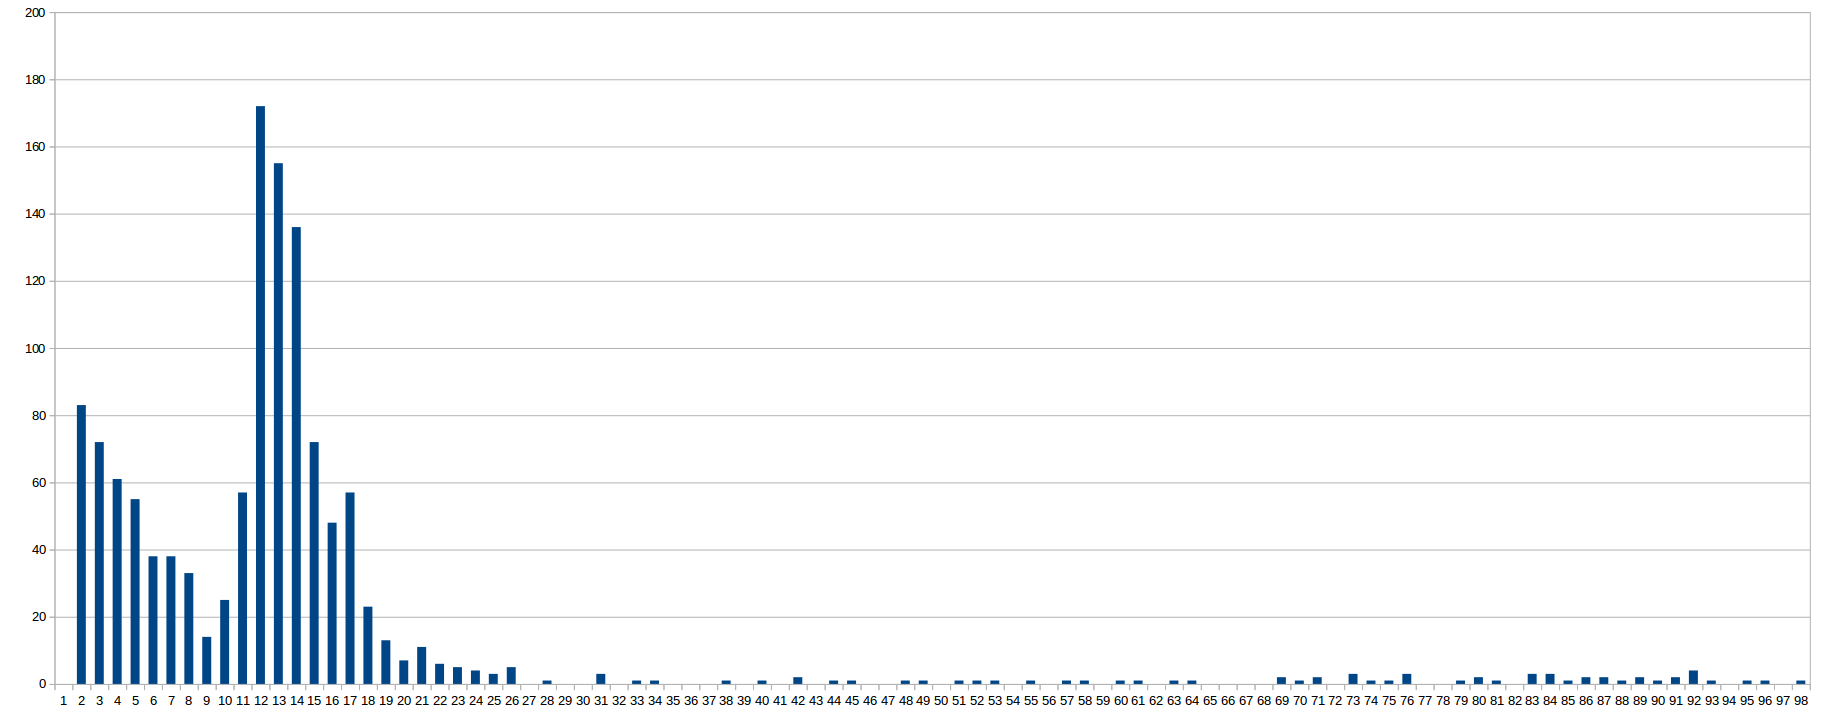
\includegraphics[scale=.17]{./uniform.png}
        \caption{Sampled (uniform law) degree distribution of the subnetwork}
        \label{fig:uniform}
\end{figure}

The two maxima have not the same importance in the total degree distribution and in the sampled one. Indeed, with the random walk, we spend statistically more time in the "core" of the network.

%-------------------------------------------------------------------------------------------------------%
\section*{Question 6}
Then, it's sufficient to implement the \textit{monteCarlo} method : \\

\medbreak
\noindent     \textit{\# choose a node following the Monte Carlo rule}\\
\noindent     \texttt{def monteCarlo(matrix,line):}\\
\hspace*{1cm} \texttt{	l = len(line)}\\
\hspace*{1cm} \texttt{	neighbourNumber = sum(nodeDegree(matrix,line))}\\
\hspace*{1cm} \texttt{	listProba = list()}\\
\hspace*{1cm} \texttt{	for i in range(0,l):}\\
\hspace*{2cm} \texttt{		listNodes = list()}\\
\hspace*{2cm} \texttt{		listNodes.append(line[i])}\\
\hspace*{2cm} \texttt{		p = float(nodeDegree(matrix,listNodes)[0])/float(neighbourNumber)}\\
\hspace*{2cm} \texttt{		listProba.append(p)}\\
\hspace*{1cm} \texttt{	normalisation = 0}\\
\hspace*{1cm} \texttt{	for i in range(0,l):}\\
\hspace*{2cm} \texttt{		listProba[i]=1./float(listProba[i])}\\
\hspace*{2cm} \texttt{		normalisation += listProba[i]}\\
\hspace*{1cm} \texttt{	for i in range(0,l):}\\
\hspace*{2cm} \texttt{		listProba[i] = float(listProba[i])/float(normalisation)}\\
\hspace*{1cm} \texttt{	for i in range(1,l):}\\
\hspace*{2cm} \texttt{		listProba[i]+=listProba[i-1]}\\
\hspace*{1cm} \texttt{	a = random.random()}\\
\hspace*{1cm} \texttt{	for i in range(0,l):}\\
\hspace*{2cm} \texttt{		if(a<listProba[i]):}\\
\hspace*{3cm} \texttt{			return line[i]}\\
\hspace*{1cm} \texttt{	return line[l]}\\
\medbreak

Then, we just have to call \texttt{randomWalk(ADJ,G,N0,400,monteCarlo)}, and we get the \textsc{Figure} \ref{fig:montecarlo}.

\begin{figure}[!h]
        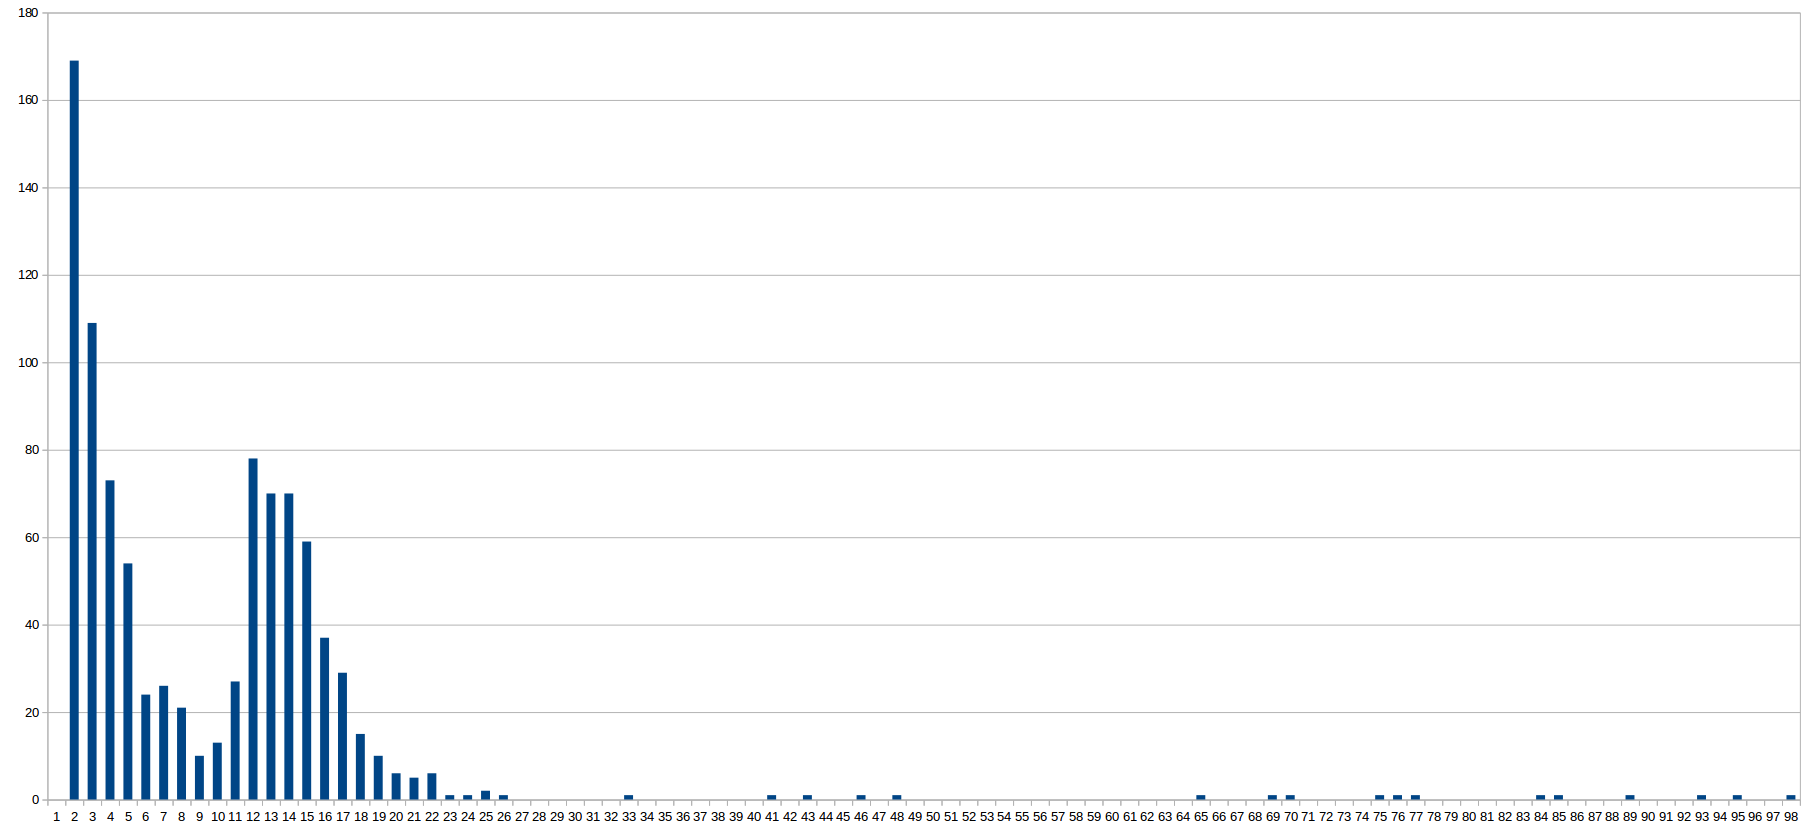
\includegraphics[scale=.17]{./montecarlo.png}
        \caption{Sampled (Monte Carlo method) degree distribution of the subnetwork}
        \label{fig:montecarlo}
\end{figure}

By forcing to explore the less dense areas of the network, the shape of the new sampled degree distribution is closer to the total one.

%-------------------------------------------------------------------------------------------------------%
\section*{Question 7}
Thanks to \texttt{networkx}, we have the \textsc{Figure} \ref{fig:subnetwork}.

\begin{figure}[!h]
        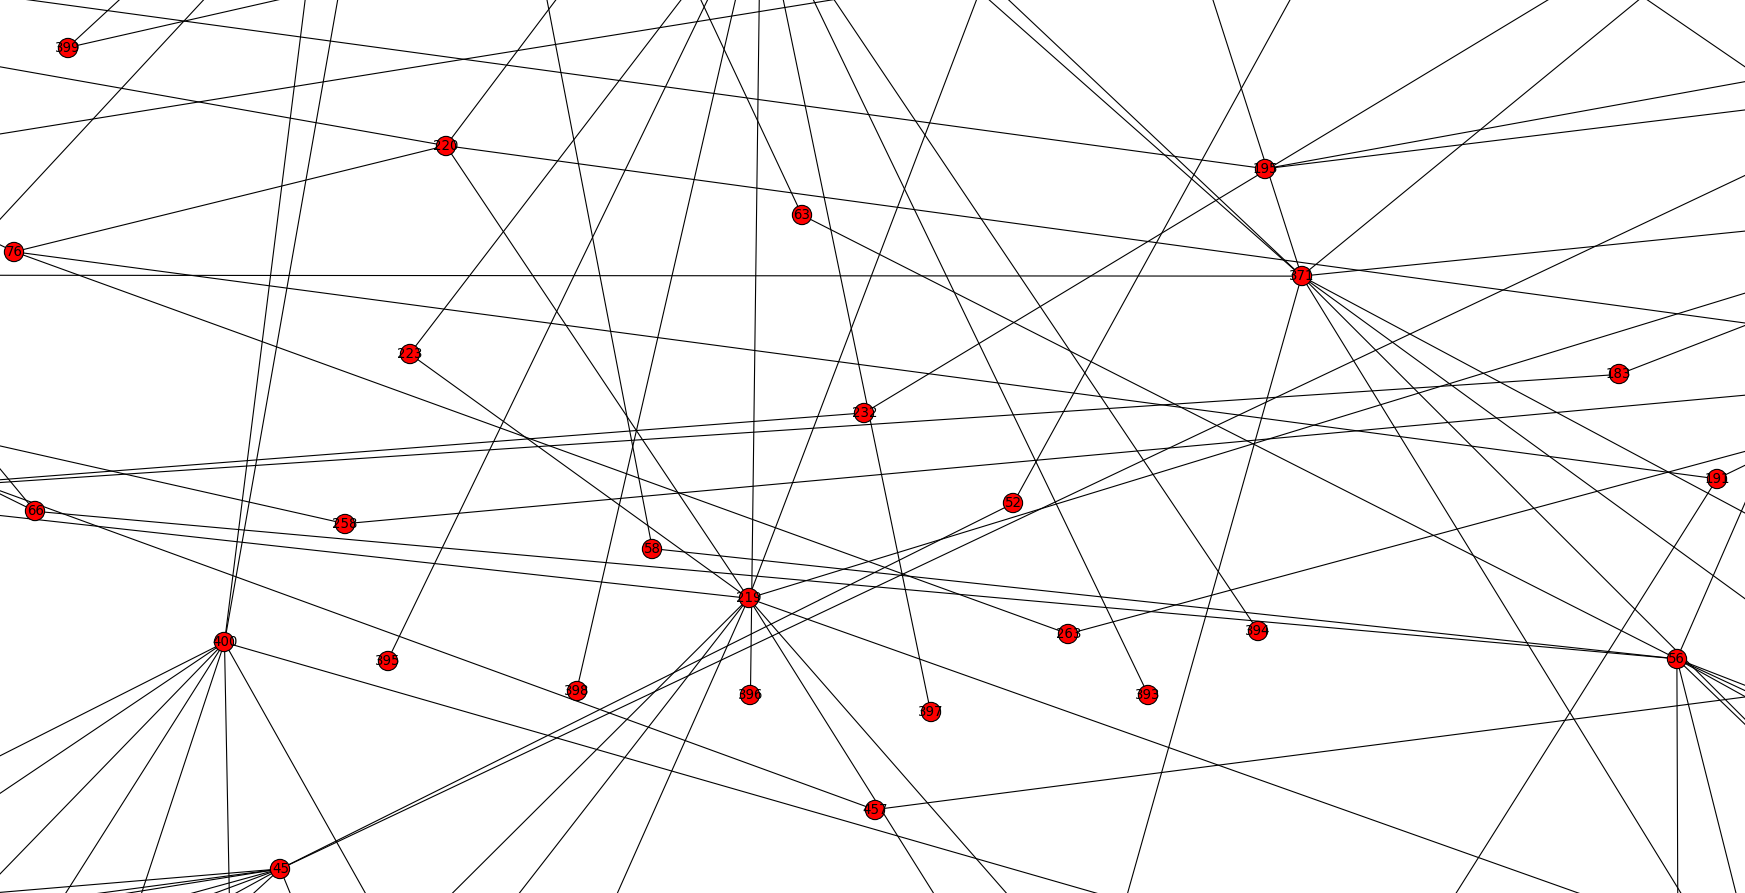
\includegraphics[scale=.2]{./subnetwork.png}
        \caption{Sample of the subnetwork}
        \label{fig:subnetwork}
\end{figure}

%-------------------------------------------------------------------------------------------------------%
\section*{Question 8}
The \textit{diameter} of the subnetwork is $D_S=13$.
\medbreak
We could pick randomly two nodes, compute the distance.
If we iterate many times and we keep the maximum of the computed distances, we should converge to the diameter.

%-------------------------------------------------------------------------------------------------------%
\section*{Question 9}
The \textit{average distance} of the subnetwork is $5.612$, which is strictly greater than $log(500)=2.699$. Thus, the subnetwork is not \textit{small world}.

%-------------------------------------------------------------------------------------------------------%
\section*{Question 10}
The first eigenvalue is $\lambda_1 = 1$. The second one is ... .
\medbreak
The smaller is the second biggest eigenvalue (all smaller than 1), the quicker is the convergence to the stationary distribution.
\end{document}
